\chapter{伊辛關聯、平均場與自發磁化}

\lectureoverview{一維伊辛鏈可透過將格點自旋改寫為鍵變數而精確求解。這項變數替換使配分函數因式分解，並顯示所有有限溫度下的關聯都呈指數衰減。高維晶格的情形不同，因為每個自旋都受到許多近鄰的影響。將近鄰的綜合影響視為平均場，便可得到自洽方程、平均場臨界溫度，並精確說明任意微弱的外場如何選定其中一個磁化相。}

\section{伊辛實際上發現了什麼}

歷史上的要點應該準確陳述。恩斯特·伊辛求解了威廉·楞次交給他的那個一維模型，並正確發現模型沒有有限溫度相變。過度推論之處，在於認為相同結論應適用於所有維度；事實並非如此。二維模型已經有有序的低溫相。

對目前的目的而言，追求高維精確解未免過於雄心勃勃。只要採用一個物理圖像清楚的近似，就足以揭示每個自旋有許多近鄰時的相變。不過，在採用這個近似之前，先精確求解一維鏈很有幫助。精確的一維答案與高維近似形成對照，指出了一維所缺少的機制。

這裡的相變不只是既有偏好逐漸增強。當溫度跨越臨界值時，平衡態會出現一種新的宏觀性質：即使移除原本用來使樣品取向的外場，非零磁化仍能持續存在。因此，計算必須回答兩個不同的問題：遠處的自旋是否記得某個選定自旋的取向？無窮小的場能否使任意大的樣品形成有序狀態？

\section{作為通用基礎的單自旋}

取一個二態變數
\begin{equation}
\sigma=\pm1,
\end{equation}
並採用以下能量約定：
\begin{equation}
E(\sigma)=-J\sigma,
\qquad J>0.
\end{equation}
因此，態\(\sigma=+1\)的能量較低。參數\(J\)可以代表磁矩與外加場的乘積，但此處的計算只涉及這個乘積。

將這個自旋視為與其餘系統處於熱平衡的小子系統。它的配分函數為
\begin{align}
z
&=\sum_{\sigma=\pm1}e^{-\beta E(\sigma)}
 =\sum_{\sigma=\pm1}e^{\beta J\sigma} \\
&=e^{\beta J}+e^{-\beta J}
 =2\cosh(\beta J).
\end{align}

同樣的結果也可以推廣到由\(N\)個獨立自旋組成的系統。完整配分函數就是\(Z=z^N\)，因此\(\log Z=N\log z\)，每個廣延熱力學量也都是單一自旋相應量的\(N\)倍。這種子系統的觀點取代了逐一計算朝上與朝下自旋數目的繁複組合計數，但兩者包含相同資訊。
平均能量可由對數導數求得：
\begin{align}
\expect{E}
&=-\frac{\partial}{\partial\beta}\log z \\
&=-J\frac{\sinh(\beta J)}{\cosh(\beta J)}
 =-J\tanh(\beta J).
\end{align}
由於\(E=-J\sigma\)，
\begin{equation}
\expect{\sigma}=\tanh(\beta J).
\end{equation}

\begin{figure}[ht]
\centering
\includegraphics[width=0.80\textwidth]{lecture_09_figure_02.png}
\caption{以雙曲正切形式表示的單自旋能量與磁化。}
\lectureframe{00:10:06}
\end{figure}

這個公式同時涵蓋兩個溫度極限。低溫時，\(\beta J\gg1\)，自旋幾乎必定處於能量較低的態。高溫時，\(\beta J\ll1\)，因此
\begin{equation}
\expect{\sigma}\simeq \beta J\longrightarrow0.
\end{equation}
熱擾動會抹平能量上的偏好。

\begin{classroomqa}
\audiencequestion{平均能量應該帶負號嗎？}
\lecturerresponse{是的。熱力學恆等式為\(\expect{E}=-\partial_\beta\log z\)，所以結果是\(-J\tanh(\beta J)\)。再除以\(-J\)，也就是\(E=-J\sigma\)中的因子，便得到正的磁化\(\expect{\sigma}=\tanh(\beta J)\)。\lecturetimestamp{00:09:15--00:09:44}}
\end{classroomqa}

\section{一維鏈}

將\(N\)個自旋置於開鏈上，並令相鄰自旋彼此作用：
\begin{equation}
H=-J\sum_{i=1}^{N-1}\sigma_i\sigma_{i+1},
\qquad \sigma_i=\pm1.
\label{eq:ising-chain}
\end{equation}
當\(J>0\)時，平行自旋對的能量貢獻為\(-J\)，反平行自旋對的貢獻則為\(+J\)。因此，兩個基態為
\begin{equation}
(+,+,\ldots,+)
\qquad\text{and}\qquad
(-,-,\ldots,-).
\end{equation}

\begin{figure}[ht]
\centering
\includegraphics[width=0.80\textwidth]{lecture_09_figure_03.png}
\caption{開鏈的哈密頓量及其玻爾茲曼加權總和。}
\lectureframe{00:19:15}
\end{figure}

將\(J\)改為\(-J\)會使交替排列的自旋較穩定。在開鏈或偶數長度的週期鏈上，重新定義
\begin{equation}
\widetilde{\sigma}_i=(-1)^i\sigma_i
\end{equation}
便能將反鐵磁耦合的符號轉換回鐵磁耦合的符號。兩者在物理上有所區別，但一維配分函數的代數推導相同。奇數長度的週期鏈是常見的例外，因為若不產生挫折，就無法讓自旋交替排列。

\begin{classroomqa}
\audiencequestion{鏈的哈密頓量中有外加磁場嗎？}
\lecturerresponse{還沒有。式~\eqref{eq:ising-chain}只包含最近鄰耦合。稍後會加入均勻外場作為獨立項，\(-h\sum_i\sigma_i\)，藉此檢驗有序態如何回應任意微弱的偏置。\lecturetimestamp{00:18:54--00:19:13}}
\end{classroomqa}

\subsection{以關聯函數衡量記憶}

假設已知\(\sigma_i\)朝上。這項資訊會影響相隔\(r\)個鍵的自旋嗎？判斷方式是計算
\begin{equation}
C(r)=\expect{\sigma_i\sigma_{i+r}}.
\end{equation}
若\(C(r)\)在\(r\to\infty\)時趨近非零值，表示系統保有長程記憶；若它趨近零，則第一個自旋的影響終究會消失。

傳話遊戲提供了恰當的直覺。每個人都把一個二進位符號傳給下一個人。如果每次傳遞都完美無誤，最初的位元便會一直保留下來。如果每一步都有非零的出錯機率，反覆傳遞終究會讓原始訊息遺失。零溫度就是伊辛鏈完美傳遞的極限。只要溫度高於零，相鄰自旋就可能偶爾不一致。

例如，假設單次傳遞的保真度為\(0.99\)。連續兩次傳遞都完美無誤的機率是\(0.99^2=0.9801\)，每多傳一步就再乘上一個\(0.99\)。傳一百步，出錯就已很常見；傳一萬步，實際上便無法保留記憶。伊辛鏈使用的是保真度的帶符號量，而非「完全無誤」的機率，但兩者的乘法式衰減概念相同。

只要區分機率與關聯，這個類比就完全成立。若\(p\)是相鄰自旋一致的機率，則
\begin{equation}
\expect{\sigma_i\sigma_{i+1}}
=p-(1-p)=2p-1.
\end{equation}
因此，沿著每個鍵相乘的量是超出隨機基準的保真度\(2p-1\)，而不是\(p\)本身。

\section{鍵變數與精確配分函數}

關鍵的變數替換，是改以自旋之間的關係來描述系統：
\begin{equation}
\mu_i=\sigma_i\sigma_{i+1},
\qquad i=1,\ldots,N-1.
\label{eq:bond-variable}
\end{equation}
自旋一致時，鍵變數為\(+1\)；不一致時則為\(-1\)。若固定第一個自旋，這些鍵變數便能決定其餘每個自旋：
\begin{align}
\sigma_2&=\sigma_1\mu_1,\\
\sigma_3&=\sigma_1\mu_1\mu_2,\\
\sigma_{r+1}&=\sigma_1\prod_{k=1}^{r}\mu_k.
\end{align}
沒有冗餘資訊。資料\((\sigma_1,\mu_1,\ldots,\mu_{N-1})\)與\((\sigma_1,\ldots,\sigma_N)\)等價。

用這些變數表示，能量便是
\begin{equation}
H=-J\sum_{i=1}^{N-1}\mu_i.
\end{equation}
原本彼此作用的格點自旋，現在變成彼此獨立的鍵變數。先對\(\sigma_1\)的兩個可能值求和，可得
\begin{align}
Z_N
&=2\sum_{\{\mu_i=\pm1\}}
\exp\left(\beta J\sum_{i=1}^{N-1}\mu_i\right)\\
&=2\prod_{i=1}^{N-1}
\left(\sum_{\mu_i=\pm1}e^{\beta J\mu_i}\right)\\
&=2\left[2\cosh(\beta J)\right]^{N-1}.
\label{eq:chain-partition}
\end{align}
總共有\(N-1\)個因子，因為有\(N\)個格點的開鏈包含\(N-1\)個鍵。

最前面的因子二，來自第一個自旋的全域選擇。它對\(\log Z_N\)只貢獻\(\log2\)；鍵變數則貢獻一個與\(N-1\)成正比的項。這個因子對精確的有限尺寸計數很重要，但當\(N\to\infty\)時，便不影響自由能密度。因此，板書上說它「沒什麼大不了」，並不代表真的把它省略了。

\begin{figure}[ht]
\centering
\includegraphics[width=0.82\textwidth]{lecture_09_figure_04.png}
\caption{將格點哈密頓量改寫為獨立鍵變數的總和，以及因此得到的因式分解配分函數。}
\lectureframe{00:35:35}
\end{figure}

\begin{classroomqa}
\audiencequestion{指數中的總和在最後答案變成乘冪時，去了哪裡？}
\lecturerresponse{它先變成乘積，才進一步化為乘冪：
\[
e^{\beta J\sum_i\mu_i}=\prod_i e^{\beta J\mu_i}.
\]
對所有鍵構形求和後，便分解為每個鍵各自的一個二項和。每個因子都是\(2\cosh(\beta J)\)，所以乘積就是它的\((N-1)\)次方。將三個自旋、兩個鍵的情形逐項寫出，因式分解便一目了然。\lecturetimestamp{00:33:25--00:35:36}}
\end{classroomqa}

這是一種簡單的對偶描述：格點上的耦合變數，換成了鍵上的非耦合變數。\emph{對偶}一詞用得恰當，因為同一個系統可以有兩種自由度面貌迥異的描述。此處的對偶，是針對一維開鏈所作的精確變數替換。

以晶格的語言來說，原始變數位於頂點，新變數則位於邊。要從邊變數重建頂點自旋，只需額外知道第一個自旋的全域選擇。這種格點與鍵之間的轉換，只是某種模式的簡單例子；到了高維統計力學中，這種模式會變得強大得多。

\subsection{最近鄰保真度}

每個鍵的機率分布都相同：
\begin{equation}
\begin{aligned}
\Pr(\mu=+1)&=\frac{e^{\beta J}}{2\cosh(\beta J)},\\
\Pr(\mu=-1)&=\frac{e^{-\beta J}}{2\cosh(\beta J)}.
\end{aligned}
\end{equation}
因此，
\begin{equation}
\expect{\mu_i}
=\expect{\sigma_i\sigma_{i+1}}
=\tanh(\beta J).
\label{eq:nearest-correlation}
\end{equation}

\begin{figure}[ht]
\centering
\includegraphics[width=0.80\textwidth]{lecture_09_figure_05.png}
\caption{以鍵變數的平均值表示最近鄰關聯。}
\lectureframe{00:36:52}
\end{figure}

因此，相鄰自旋一致的機率為
\begin{equation}
p_{\rm same}
=\frac{1+\tanh(\beta J)}{2}.
\end{equation}
當\(J\)為正值時，這個機率大於二分之一；零溫度時趨近於一；無限高溫時則為二分之一。

\begin{classroomqa}
\audiencequestion{為什麼最近鄰關聯為正，表示自旋偏好同向排列，而不是反向排列？}
\lecturerresponse{當\(J>0\)時，同向鍵的能量為\(-J\)，反向鍵的能量為\(+J\)。\(\expect{\mu}\)為正表示\(\mu=+1\)較常出現，也就是同向排列較常出現。真實材料的有效耦合屬於鐵磁或反鐵磁，取決於其微觀電子結構；此處採用的符號約定描述的是鐵磁體。\lecturetimestamp{00:43:45--00:44:48}}
\end{classroomqa}

\begin{classroomqa}
\audiencequestion{溫度非常高時，這個關聯會如何變化？}
\lecturerresponse{當\(T\to\infty\)時，\(\beta\to0\)，而且\(\tanh(\beta J)\to0\)。此時即使最近鄰也不再彼此攜帶任何資訊：每個自旋都像是在隨機猜測。\lecturetimestamp{00:46:42--00:47:20}}
\end{classroomqa}

\subsection{長程關聯}

相隔\(r\)個鍵的兩個自旋，其關聯為
\begin{align}
\sigma_i\sigma_{i+r}
&=\sigma_i
\left(\prod_{k=i+1}^{i+r-1}\sigma_k^2\right)
\sigma_{i+r}\\
&=(\sigma_i\sigma_{i+1})
(\sigma_{i+1}\sigma_{i+2})\cdots
(\sigma_{i+r-1}\sigma_{i+r})\\
&=\prod_{k=i}^{i+r-1}\mu_k.
\end{align}
由於\(\mu_k\)彼此獨立，
\begin{equation}
C(r)=\expect{\sigma_i\sigma_{i+r}}
=\left[\tanh(\beta J)\right]^r.
\label{eq:exact-correlation}
\end{equation}

\begin{figure}[ht]
\centering
\includegraphics[width=0.80\textwidth]{lecture_09_figure_06.png}
\caption{中間插入的\(\sigma_k^2=1\)因子，將遠距自旋的乘積改寫成獨立鍵變數的乘積。}
\lectureframe{00:41:35}
\end{figure}

\begin{classroomqa}
\audiencequestion{關聯函數只包含兩端的自旋。所有中間自旋是從哪裡來的？}
\lecturerresponse{它們只是以等於一的因子插入：\(\sigma_k^2=1\)。將相鄰的自旋因子兩兩配對，就能把兩端自旋的乘積改寫為鍵變數；這些鍵變數的熱分布正好可以因式分解。關聯函數的值並未改變。\lecturetimestamp{00:41:41--00:42:26}}
\end{classroomqa}

在任何有限溫度下，
\begin{equation}
0<\tanh(\beta J)<1,
\end{equation}
記憶因此呈指數衰減。令
\begin{equation}
C(r)=e^{-r/\xi}
\end{equation}
便可定義精確的關聯長度
\begin{equation}
\xi^{-1}=-\log\!\left[\tanh(\beta J)\right].
\label{eq:correlation-length}
\end{equation}
只有在\(T=0\)時，\(\xi\)才會發散。在低但非零的溫度下，
\begin{equation}
\xi\simeq \frac{1}{2}e^{2\beta J},
\end{equation}
因此，鏈上可以有非常長的自旋同向區段，卻仍不具備真正的無限程有序。

因此，這條鏈看起來像是由一段段區域組成：先是一長串朝上的自旋，接著翻轉，再來一長串朝下的自旋，然後又翻轉。低溫會讓這些區段變長，因為疇壁很少見；但疇壁並未完全消失。磁化需要無限長的記憶長度，而不只是非常大的記憶長度。

\section{為何更多近鄰會改變問題}

一維沒有糾錯能力。某個鍵一旦與前一個鍵不一致，下一個自旋便沒有其他獨立資訊來源可告知它原本應該朝哪個方向。因此，這條鏈由長段的同向自旋區域組成，偶爾才會發生翻轉。

正方晶格中，每個格點有四個最近鄰；立方晶格中則有六個。在\(d\)維超立方晶格中，每個格點有
\begin{equation}
z=2d
\end{equation}
個最近鄰。若某個格點接收到三個一致的訊號和一個不一致的訊號，它就可以依從多數。近鄰眾多的環境能抑制孤立錯誤，原理很像透過冗餘訊息來糾錯。

若近鄰的平均自旋為\(m\)，它們的總和平均為\(zm\)。其典型漲落量級為\(\sqrt{z}\)，因此遠離\(m=0\)時，相對漲落大致按下式變化：
\begin{equation}
\frac{\sqrt{z}}{z|m|}
=\frac{1}{\sqrt{z}\,|m|}.
\end{equation}
這說明為什麼配位數很大時，平均場近似變得合理。另一方面，這也提醒我們，在臨界點附近\(m\)很小，此近似最不可靠。

有句俗話道出了大數量的直覺：一百張獨立選票不太可能全都朝同一方向投錯。其定量描述就是平方根定律。\(z\)個變數中的一致偏向與\(z\)成正比，而隨機不一致通常只與\(\sqrt{z}\)成正比。因此，維度提高不只增加近鄰數，也會改變近鄰集體訊息的可靠性。

\begin{classroomqa}
\audiencequestion{高於三維的維度是否對應到真實的磁性材料？}
\lecturerresponse{若把它們視為空間維度，則不能直接對應。\(d\)很大時，便是每個格點都有許多近鄰、平均化可以受到控制的可解極限。在這個極限看清機制後，就可以進一步探問它在多大程度上仍適用於物理維度。對伊辛模型而言，二維已足以出現有限溫度相變，雖然平均場無法給出二維的精確答案。\lecturetimestamp{00:52:32--00:53:50}}
\end{classroomqa}

\section{將平均場視為自洽問題}

考慮一個自旋\(\sigma_i\)。它與\(z=2d\)個近鄰之間的交互作用為
\begin{equation}
E_i=-J\sigma_i\sum_{j\in{\rm nn}(i)}\sigma_j.
\label{eq:local-energy}
\end{equation}
令
\begin{equation}
m=\expect{\sigma}
\end{equation}
表示每個自旋的均勻平均磁化。平均場將波動的近鄰自旋總和替換為其平均值：
\begin{equation}
\sum_{j\in{\rm nn}(i)}\sigma_j
\longrightarrow zm=2dm.
\end{equation}
於是，這個選定自旋的有效單自旋能量為
\begin{equation}
E_i^{\rm MF}=-2dJm\,\sigma_i.
\label{eq:mean-field-energy}
\end{equation}

\begin{figure}[ht]
\centering
\includegraphics[width=0.82\textwidth]{lecture_09_figure_07.png}
\caption{選定的自旋、它的\(2d\)個最近鄰，以及以平均磁化替換近鄰自旋總和的示意圖。}
\lectureframe{01:00:30}
\end{figure}

現在可以把有效場\(2dJm\)代入單自旋結果：
\begin{equation}
\expect{\sigma_i}_{\rm effective}
=\tanh(2\beta dJm).
\end{equation}
但這個格點並沒有特殊之處。平移不變性要求它的平均值等於原先假設的平均值\(m\)。因此，
\begin{equation}
\boxed{m=\tanh(2\beta dJm)}.
\label{eq:self-consistency}
\end{equation}
這就是平均場也稱為自洽場近似的原因：產生有效場的磁化，必須等於該有效場所產生的磁化。

\begin{classroomqa}
\audiencequestion{有效單自旋的結果中是不是漏了\(\beta\)？}
\lecturerresponse{這個因子不能省略。指數函數或雙曲正切函數的引數必須是無因次的，因此有效能量\(2dJm\)必須以\(2\beta dJm\)的形式出現。\lecturetimestamp{01:00:13--01:00:27}}
\end{classroomqa}

\begin{classroomqa}
\audiencequestion{這個方程是否只表示\(m\)與自身成正比？}
\lecturerresponse{不是。未知的磁化出現在非線性函數內：
\[
m=\tanh(2\beta dJm).
\]
這是隱式方程，依溫度而定，可能有一個或多個解。\lecturetimestamp{01:02:12--01:02:42}}
\end{classroomqa}

\begin{classroomqa}
\audiencequestion{這個自洽方程是否假設高溫，或假設雙曲正切的引數很小？}
\lecturerresponse{不是。方程\(m=\tanh(2\beta dJm)\)是適用於所有溫度的完整平均場方程。只有後續採用\(\tanh x\simeq x\)這類近似時，才需要\(x\)很小；這種近似會在臨界點附近用來求出或展開新出現的解。\lecturetimestamp{01:02:44--01:03:12}}
\end{classroomqa}

\begin{classroomqa}
\audiencequestion{上方橫線的記號和一般的尖括號平均不同嗎？}
\lecturerresponse{沒有不同。板書上的橫線是熱平均的簡寫：\(\bar{\sigma}=\expect{\sigma}=m\)。\lecturetimestamp{01:03:19--01:03:42}}
\end{classroomqa}

\begin{classroomqa}
\audiencequestion{\(2d\)個自旋都是最近鄰嗎？更遠距離的耦合也會有類似效果嗎？}
\lecturerresponse{在超立方晶格上，是的：沿著\(d\)個座標軸，每個軸都有兩個最近鄰。次近鄰及更遠距離的耦合屬於不同的模型，通常各有其耦合強度；不過，增加交互作用範圍也會提高有效配位數，讓平均場推理更加準確。\lecturetimestamp{01:03:43--01:05:12}}
\end{classroomqa}

\section{以圖形描繪相變}

定義
\begin{equation}
K=2\beta dJ,
\qquad
y=Km.
\end{equation}
則式~\eqref{eq:self-consistency}可改寫為
\begin{equation}
\frac{y}{K}=\tanh y.
\label{eq:graph-equation}
\end{equation}
右側是固定的 S 形曲線。左側則是通過原點的直線，其斜率為
\begin{equation}
\frac{1}{K}=\frac{T}{2dJ},
\end{equation}
其中\(k_{\rm B}=1\)。

高溫時，直線較陡，與\(\tanh y\)只在\(y=0\)處相交。低溫時，直線較平緩，有三個交點：\(y=0\)以及一對對稱的\(y=\pm y_0\)。臨界門檻出現在直線與\(\tanh y\)於原點的斜率相同時。由於\(\tanh'(0)=1\)，
\begin{equation}
K_c=1,
\qquad
T_c^{\rm MF}=2dJ.
\label{eq:mean-field-tc}
\end{equation}
這是平均場臨界溫度，並非低維系統的精確答案。

假設\(J>0\)表示相鄰自旋偏好一致，但並未在\(+m\)與\(-m\)之間擇一。在零外場下，哈密頓量在全域自旋翻轉\(\sigma_i\mapsto-\sigma_i\)之下不變，因此兩個非零交點在物理上等價。只畫圖的正半部，是為了方便呈現，並不代表負磁化相不存在。

\begin{figure}[ht]
\centering
\includegraphics[width=0.82\textwidth]{lecture_09_figure_08.png}
\caption{直線族與\(\tanh y\)：高溫時有一個交點，低溫時有三個交點。}
\lectureframe{01:11:50}
\end{figure}

\begin{figure}[ht]
\centering
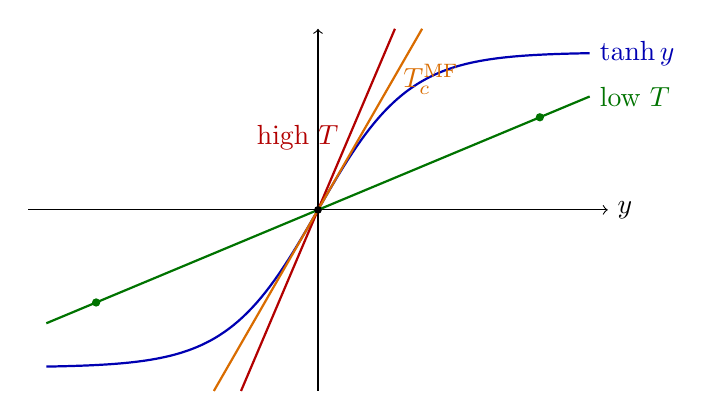
\begin{tikzpicture}[x=1.15cm,y=2.0cm]
\draw[->] (-3.2,0) -- (3.2,0) node[right] {$y$};
\draw[->] (0,-1.15) -- (0,1.15);
\draw[thick,blue!70!black,domain=-3:3,samples=120]
  plot (\x,{tanh(\x)}) node[right] {$\tanh y$};
\draw[thick,red!70!black] (-0.85,-1.15) -- (0.85,1.15)
  node[pos=0.70,left] {high \(T\)};
\draw[thick,orange!85!black] (-1.15,-1.15) -- (1.15,1.15)
  node[pos=0.86,right] {\(T_c^{\rm MF}\)};
\draw[thick,green!45!black] (-3,-0.72) -- (3,0.72)
  node[right] {low \(T\)};
\fill (0,0) circle (1.4pt);
\fill[green!45!black] (-2.45,-0.588) circle (1.5pt);
\fill[green!45!black] (2.45,0.588) circle (1.5pt);
\end{tikzpicture}
\caption{以圖形重現自洽論證，並將數值歸一化。}
\end{figure}

非零分支會連續出現。在相變附近，
\begin{equation}
\tanh(Km)=Km-\frac{(Km)^3}{3}+O(m^5).
\end{equation}
當\(K>1\)時，小的非零解滿足
\begin{equation}
m^2\simeq \frac{3(K-1)}{K^3}.
\end{equation}
因此，平均場預測磁化會以熟悉的平方根形式開始增長：\(m\propto(T_c-T)^{1/2}\)。

不必依賴圖形，也能陳述穩定性。忽略與\(m\)無關的常數後，每個自旋的平均場自由能為
\begin{equation}
f_{\rm MF}(m)
=dJm^2-\frac{1}{\beta}
\log\!\left[2\cosh(2\beta dJm)\right].
\label{eq:mf-free-energy}
\end{equation}
其駐點條件為
\begin{equation}
\frac{\partial f_{\rm MF}}{\partial m}
=2dJ\left[m-\tanh(2\beta dJm)\right]=0.
\end{equation}
高於\(T_c^{\rm MF}\)時，\(m=0\)是極小值；低於臨界溫度時，原點是局部極大值，而兩個非零解是簡併的極小值。交點的幾何與自由能的熱力學分析，給出相同結論。

\begin{classroomqa}
\audiencequestion{在\(T_c^{\rm MF}\)以下，解\(m=0\)仍是交點。為什麼非零分支才是物理解？}
\lecturerresponse{從零溫度逐漸升高，系統原本就在磁化分支上。更形式地說，在相變溫度以下，平均場自由能在\(\pm m_0\)處有極小值，而\(m=0\)則成為極大值。此時，無窮小的外場會選定其中一個極小值，消除表面上的歧義。\lecturetimestamp{01:11:34--01:12:18}}
\end{classroomqa}

\section{為什麼一維使平均場失效}

將\(d=1\)代入式~\eqref{eq:mean-field-tc}，會預測相變發生於\(T=2J\)，與精確的一維解相矛盾。這裡沒有任何代數量發散。近似失效的原因是：兩個近鄰不足以構成大型統計熱浴，而且一維疇壁的熵有其特殊之處。

從所有自旋朝上的狀態開始。斷鍵會使能量從\(-J\)變成\(+J\)，因此每個斷鍵的能量代價為
\begin{equation}
\Delta E_{\rm bond}=2J.
\end{equation}
在正方晶格上，翻轉一個自旋會斷開四個鍵，代價為\(8J\)。若翻轉的兩個自旋相鄰，周界有六個斷鍵，代價為\(12J\)；若兩個翻轉自旋相距甚遠，則會斷開八個鍵，代價為\(16J\)。

\begin{figure}[ht]
\centering
\includegraphics[width=0.82\textwidth]{lecture_09_figure_09.png}
\caption{正方晶格上兩個相鄰的反轉自旋；兩者共用的鍵仍滿足排列條件，周界因此有六個斷鍵。}
\lectureframe{01:17:30}
\end{figure}

因此在二維中，緊湊的反轉自旋區域所需付出的能量與其邊界長度成正比：
\begin{equation}
\Delta E_{\rm 2d}=2J\,|\partial D|.
\end{equation}
區域通常越大，邊界也越長。

一維則不同。無論連續反轉的自旋區域有多長，都只有兩個疇壁：
\begin{equation}
\Delta E_{\rm 1d}=2(2J)=4J.
\label{eq:one-d-domain-cost}
\end{equation}

\begin{figure}[ht]
\centering
\includegraphics[width=0.82\textwidth]{lecture_09_figure_10.png}
\caption{一維中一段很長的反轉自旋區域，僅由兩個疇壁界定。}
\lectureframe{01:19:10}
\end{figure}

在有\(N\)個格點的鏈上，這種區域的兩個疇壁約有\(N^2\)種選法。兩壁之間的距離增加，並不會提高其能量。在任何正溫度下，熵因此都會使任意大的反轉區域得以出現。在二維中，低溫時的邊界能量則可以壓過輪廓熵。這種能量與熵之間的競爭，正是平均場無法看見的幾何事實；平均場只把\(d=1\)與\(d=2\)視為同一係數的不同數值。

\begin{classroomqa}
\audiencequestion{固定的雙壁能量代價是否要求翻轉的自旋彼此相鄰？}
\lecturerresponse{是的。這裡討論的是一段連續的反轉自旋區域。若翻轉的自旋分成數段彼此分離的區域，每段都會多出兩個疇壁。關鍵在於，單一區域可以任意長，卻始終只有兩個疇壁。\lecturetimestamp{01:18:32--01:18:40}}
\end{classroomqa}

\begin{classroomqa}
\audiencequestion{平均場方程本身似乎沒有呈現\(d=1\)與\(d=2\)之間的定性差異。問題就在這裡嗎？}
\lecturerresponse{正是如此。平均場預測任何正的\(d\)都會發生相變，因此對一維而言，定性上就是錯的。推導時假設近鄰很多且漲落微弱，並忽略了疇壁的幾何效應。一維的情形應由精確的鍵變數解來判定，而不是依靠平均場替換\(d=1\)。\lecturetimestamp{01:19:44--01:20:28}}
\end{classroomqa}

\section{外場選定相}

加入均勻外場\(h\)，並約定當\(h>0\)時，\(\sigma=+1\)較有利：
\begin{equation}
H=-J\sum_{\langle ij\rangle}\sigma_i\sigma_j
-h\sum_i\sigma_i.
\label{eq:ising-with-field}
\end{equation}
選定自旋的平均場能量為
\begin{equation}
E_i^{\rm MF}=-(2dJm+h)\sigma_i,
\end{equation}
自洽方程則變為
\begin{equation}
\boxed{m=\tanh\!\left[\beta(2dJm+h)\right]}.
\label{eq:self-consistency-field}
\end{equation}
令\(K=2\beta dJ\)及\(y=Km\)，
\begin{equation}
\frac{y}{K}=\tanh(y+\beta h).
\label{eq:shifted-graph}
\end{equation}

\begin{figure}[ht]
\centering
\includegraphics[width=0.82\textwidth]{lecture_09_figure_11.png}
\caption{在自洽方程中加入外場項，以及相應的平移圖形。}
\lectureframe{01:26:20}
\end{figure}

\begin{classroomqa}
\audiencequestion{為什麼外場只加在雙曲正切函數的引數中？它不也應該影響左側嗎？}
\lecturerresponse{左側是設定的磁化\(m\)，也就是\(y/K\)。右側則是在總有效場\(2dJm+h\)中，計算單一自旋所得的磁化。自洽條件要求兩者相等。由於\(y=Km\)的定義保持不變，新項只會出現在函數引數\(\tanh(y+\beta h)\)中。\lecturetimestamp{01:23:46--01:26:18}}
\end{classroomqa}

\begin{classroomqa}
\audiencequestion{同樣的圖形變化，能否用移動直線來描述，而不是平移\(\tanh\)曲線？}
\lecturerresponse{可以。可以讓\(\tanh y\)保持不變，並改寫方程，使直線出現非零截距。如此得到的交點完全相同。兩種描述的差異，只在於選擇方程的哪一側作為固定圖形。\lecturetimestamp{01:35:07--01:36:26}}
\end{classroomqa}

當\(h\neq0\)時，原點不再是解。在\(T_c^{\rm MF}\)以下，任意微弱的正外場都會選定正磁化分支；負外場則會選定負磁化分支。

\begin{figure}[ht]
\centering
\includegraphics[width=0.82\textwidth]{lecture_09_figure_12.png}
\caption{微弱外場消除對稱交點，並選定其中一個磁化分支。}
\lectureframe{01:36:22}
\end{figure}

正確的陳述必須交代極限的順序。有限系統在\(h=0\)時具有自旋翻轉對稱性，因此在完整的平衡系綜中，\(\expect{m}=0\)。自發磁化定義為
\begin{equation}
m_{\rm sp}
=\lim_{h\to0^+}\lim_{N\to\infty}\expect{m}_{N,h},
\end{equation}
其中必須先取熱力學極限。將無窮小外場的符號反轉，便得到\(-m_{\rm sp}\)。總場能差與\(Nh\)成正比，因此即使外場極微弱，對宏觀樣品仍足以產生決定性影響。

相應的自由能呈現出傾斜：
\begin{equation}
f_{\rm MF}(m;h)
=dJm^2-\frac{1}{\beta}
\log\!\left[2\cosh\!\left(\beta(2dJm+h)\right)\right].
\end{equation}
在\(h=0\)時，兩個勢阱深度相同。正的\(h\)會降低正\(m\)所對應勢阱的能量，並提高負\(m\)所對應勢阱的能量。每個自旋受到的微擾可以很小，但乘上\(N\)後，總偏好便是宏觀量。

\begin{classroomqa}
\audiencequestion{如果外加磁場一直存在，磁化真的算是自發的嗎？}
\lecturerresponse{磁場的作用僅是選定一個分支。在固定 \(T<T_c\)時，先取系統的無限大極限，再令 \(h\to0^+\)。即使選相磁場消失，磁化仍保持有限。反轉極限的符號，就會選到相反的相。\lecturetimestamp{01:33:15--01:34:18}}
\end{classroomqa}

\begin{classroomqa}
\audiencequestion{在相變以下，零平均解究竟是不可能，還是只是不穩定？}
\lecturerresponse{恰在零場時，有限體積系綜可以是對稱的，並讓兩種取向具有相同權重，因此平均值為零。問題在於，這種狀態無法作為單一宏觀相保持穩定。任意微小的磁場都會改變廣延能量的平衡，並選定一種取向；取熱力學極限後，即使移除磁場，所選取向的磁化仍然存在。\lecturetimestamp{01:34:25--01:35:06}}
\end{classroomqa}

\begin{classroomqa}
\audiencequestion{在無限高溫下，受磁場偏置的解會如何？}
\lecturerresponse{對固定且有限的 \(h\)，當 \(T\to\infty\) 時，\(K=2\beta dJ\) 和 \(\beta h\) 都趨近於零。因此，方程~\eqref{eq:self-consistency-field}給出 \(m\to0\)。弱磁場可以選定低溫分支，卻無法抵抗無限強烈的熱擾動而維持有序。\lecturetimestamp{01:27:39--01:29:51}}
\end{classroomqa}

\begin{classroomqa}
\audiencequestion{溫度與圖形位移同時改變時，如何確定交點會移到哪裡？}
\lecturerresponse{直接使用隱式方程，比追著移動的草圖判斷更可靠。在低溫且 \(h\) 為正時，穩定解趨近 \(m=+1\)。在高溫下，將正切函數展開可得
\[
m\simeq \beta(2dJm+h)
\quad\Longrightarrow\quad
m\simeq \frac{\beta h}{1-2\beta dJ},
\]
當 \(\beta\to0\) 時，這個解趨近於零。因此，穩定分支從低溫下的對齊極限連接到高溫下的弱極化極限；在相變以下，它不會停留於不穩定的原點。\lecturetimestamp{01:29:53--01:33:04}}
\end{classroomqa}

\section{磁場反轉是另一個問題}

\begin{classroomqa}
\audiencequestion{是什麼使地球磁場反轉方向？}
\lecturerresponse{這個問題超出平衡伊辛模型的範圍。地球的主磁場由地球發電機產生：外核中導電流體的對流與旋轉，維持著電流和磁場。磁場反轉是這個非線性發電機系統不規則的重新組織，並非固態鐵中簡單的鐵磁疇翻轉。單一平衡序參量無法描述反轉發生的具體時序，因此坦白地說，這裡的伊辛模型計算無法解釋反轉由何觸發。兩者有用的共通之處僅在於一般原理：具有兩種相反大尺度取向的系統，可能在這兩種取向之間發生不穩定性。\footnote{參見\href{https://science.nasa.gov/science-research/earth-science/earths-magnetosphere-protecting-our-planet-from-harmful-space-energy/}{NASA 地球發電機概述}及\href{https://www.usgs.gov/programs/geomagnetism/introduction-geomagnetism}{USGS 地磁學簡介}。} \lecturetimestamp{01:38:39--01:40:32}}
\end{classroomqa}

精確解與平均場點陣模型，如今給出了截然不同的兩種答案。在一維中，
\begin{equation}
\expect{\sigma_i\sigma_{i+r}}
=\left[\tanh(\beta J)\right]^r
\longrightarrow0
\qquad (T>0),
\end{equation}
有限能量的疇壁可以將任意長的反轉區段彼此隔開，因此會得到上述結果。若鄰居數很多，自洽場則允許在
\begin{equation}
T_c^{\rm MF}=2dJ.
\end{equation}
以下存在穩定的非零解。這種差異不只是代數上的：它反映了幾何、能量、熵與冗餘之間的競爭，也就是錯誤能否自由傳播，或周圍的點陣能否將它修正。